% Mission Requirements Summary
%
The aircraft must be capable of being compactly stored, swiftly constructed, and fly various electronic warfare missions. The designed aircraft must perform three flight missions and one ground mission. Table \ref{tab:mss} provides a summary of each mission requirement.\\
%
\begin{table}[hbt!]
\caption{Mission Requirements and Subsystem Design}{\label{tab:Mss}}
\vspace*{-3mm}
\centering
\label{tab:mss}
\resizebox{\columnwidth}{!}{%
\begin{tabular}{l|l|l|l|l|}
\rowcolor{iitred}\color{white}\textbf{Mission} & \color{white}\textbf{1- Test Flight} & \color{white}\textbf{2-Assembly} & \color{white}\textbf{3-Antenna Flight} & \color{white}\textbf{4-Ground Mission} \\
\color{white}\cellcolor{iitgray}\textbf{\begin{tabular}[c]{@{}l@{}}Requirement \\Summary\end{tabular}} & \begin{tabular}[c]{@{}l@{}}No payload. Complete 3 \\ laps in 5 minutes.\end{tabular} & \begin{tabular}[c]{@{}l@{}}  Assemble the aircraft and fly as many laps as possible \\ in 10 minutes. \\ The electronics package must fly with the plane.\end{tabular} & \begin{tabular}[c]{@{}l@{}}Fly 3 laps as fast as possible\\ with the antenna attached.\end{tabular} & \begin{tabular}[c]{@{}l@{}}Structural load testing, via\\ wing-tip tes\end{tabular} \\ \hline

\color{white}\cellcolor{iitgray}\textbf{\begin{tabular}[c]{@{}l@{}}Design\\Objective\end{tabular}} & \begin{tabular}[c]{@{}l@{}}\tabitem Wing and propulsion system\\ design must enable take-off\\ in 60 ft. without EW payload\\ and provide minimum 26\\ mph average flight velocity.\end{tabular} & 

\begin{tabular}[c]{@{}l@{}} \tabitem Wing and tail boom assembly must be simple \\ and be quick to build, allowing for more flight time. \\ \tabitem Wing and tail must be secure during flight.\\ \tabitem Wing and Propulsion design should maximize cruise velocity\\ to achieve the highest amount of laps in the allotted time. \\ \tabitem Tail control surfaces should have sufficient volume to \\manage the increased weight of Electronic payload \\ and still perform attitude control duties.\end{tabular} & 
\begin{tabular}[c]{@{}l@{}} \tabitem Builds on M2’s requirements. \\ \tabitem Antenna must be mounted on wing.\\ \tabitem Tail control surfaces should be \\ capable of fixed deflection to \\ counteract surplus drag and related \\ moments caused by the antenna.\end{tabular} & 
\begin{tabular}[c]{@{}l@{}} \tabitem Structure should aim to maximize \\ wing strength to weight ratio to allow \\ for higher loading weight relative to\\ aircraft weight\end{tabular} \\ \hline

\color{white}\cellcolor{iitgray}\textbf{Scoring} & {\large $M_1 = 1.0$} (Successful) & \large $M_2 = 1 + \frac{{(Laps * W_{Payload})}_{IIT}}{{(Laps *W_{Payload})}_{max}}$ & \large $M_3 = 2 + \frac{(L_{antenna} / t)_\text{IIT}}{(L_{antenna} / t)_{max}}$ & \large $GM = \frac{(W_{total} / W_{max})_\text{IIT}}{(W_{total} / W_{max})_{max}}$ \\ \hline
\end{tabular}%
}
\end{table}

% {\renewcommand{\arraystretch}{1.25}
% \begin{atb}[H]{Mission Summary and Scoring}{tab:Mss}{>{\raggedright\arraybackslash}m{.16\linewidth} >{\raggedright\arraybackslash}m{.25\linewidth} >{\raggedright\arraybackslash}m{.25\linewidth} >{\raggedright\arraybackslash}m{.25\linewidth}}
%     %
%     % Headers
%     %
%     \makebox[\linewidth]{\centering Mission} 
%     & \makebox[\linewidth]{\centering\color{white}Summary}
%     & \makebox[\linewidth]{\centering\color{white}Design Objectives}
%     & \makebox[\linewidth]{\centering\color{white}Scoring} \\
%     %
%     % Mission 1
%     %
%     1 - Test Flight
%     & No payload. Complete 3 laps in 5 minutes.
%     & Wing and propulsion system design must take-off within 60 ft. without EW payload and provide minimum 36 mph average cruise velocity.
%     & {\large $M_1 = 1.0$} (Successful landing) \\
%     %
%     % Mission 2
%     %
%     2 - Rapid Assembly Flight
%     & \cellcolor{gray!25}Assemble the aircraft and fly as many laps as possible in 10 minutes. The electronics package must fly with the plane. 
%     & \cellcolor{gray!25} Wing and tail boom assembly must be quick to build, allowing for more flight time. Wing and tail must be secure during flight. Aircraft design should aim to maximize cruise velocity to achieve the highest amount of laps in the allotted time. Tail control surfaces should have sufficient volume to manage increased weight of EW payload and still perform attitude control duties.
%     & \cellcolor{gray!25}\large $M_2 = 1 + \frac{{(Laps * W_{Payload})}_{IIT}}{{(Laps *W_{Payload})}_{max}}$\\
%     %
%     % Mission 3
%     %
%     3 - Antenna Flight
%     & Fly 3 laps as fast as possible with the antenna attached.
%     & Builds on M2's requirements. Tail control surfaces should be capable of fixed deflection to counteract surplus drag and related moments caused by the antenna.
%     & \large $M_3 = 2 + \frac{(L_{antenna} / t)_\text{IIT}}{(L_{antenna} / t)_{max}}$ \\
%     %shorten equation to one line somehow
%     % Ground Mission
%     %
%     4 - Ground Mission
%     & \cellcolor{gray!25} Structural load testing, via wing-tip test.
%     & \cellcolor{gray!25} Structure should aim to maximize wing strength to weight ratio to allow for higher load weight to aircraft weight ratio.
%     & \cellcolor{gray!25}\large $GM = \frac{(W_{total} / W_{max})_\text{IIT}}{(W_{total} / W_{max})_{max}}$\\
% \end{atb}}

% \vspace{1cm}

\subsection{Configuration Selection} % Please edit as you see fit
A sensitivity analysis was performed to determine the effect of design parameters on score. Based on Figure \ref{fig:score_2d} and \ref{fig:score_3d} it was found that a high thrust, high payload configuration is ideal for maximizing score. It was determined that a single motor, high-wing monoplane with a conventional tail would be the most stable and highest scoring configuration. The monoplane configuration was chosen due to its low drag, low weight, and ease of manufacture. A single motor was chosen to permit increased structural strength of the wing, necessary for the Ground Mission. A high wing configuration provides higher aerodynamic stability and increases propeller sizing options.\\
% Additionally, Figure \ref{fig:score_3d} relates the geometric parameters to minimum required thrust-to-weight ratio (TWR). According to Figure \ref{fig:score_3d}, TWR is independent of wing loading, and the ideal lift coefficient is around 0.5-0.8 with highest possible wing loading. 
  \begin{figure}[htb!]
    % \vspace{-1.5em}
    % \hspace{\fill}
    \begin{subfigure}[b]{0.49\textwidth}
        \centering
        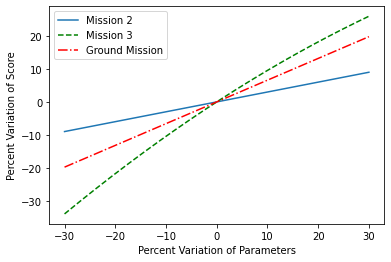
\includegraphics[width=\textwidth]{Images/DBF Mission Variation.png}
        \caption{Parameter Score Variation}
        \label{fig:score_2d}
    \end{subfigure}
    % \hspace{\fill}
    \begin{subfigure}[b]{0.49\textwidth}
        \centering
        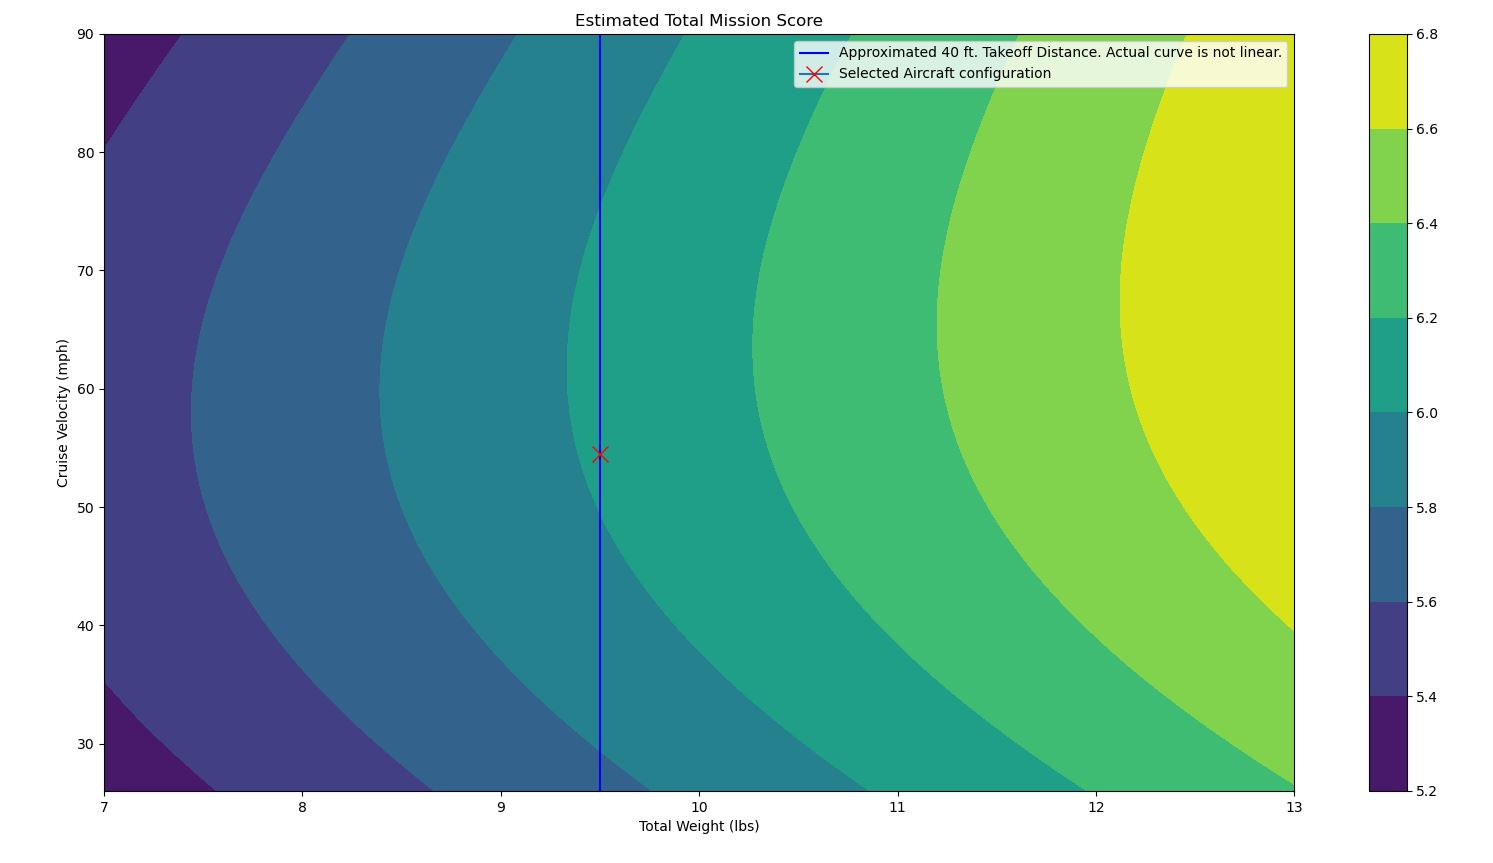
\includegraphics[width=\textwidth, height=5.5cm]{Images/final_selection_graph.JPG}
        \caption{Relating Critical Design Parameters. Line of 40 ft. Maximum takeoff distance is a linear approximation.}
        \label{fig:score_3d}
    \end{subfigure}
    % \hspace{\fill}
    \caption{Score Analysis}
    \label{fig:scoring}
    % \vspace{1em}
\end{figure}
\subsection{Preliminary Sizing}
Wing and tail dimensions were determined using XFLR5, an X-FOIL based aircraft design and analysis software. The maximum wing span of 4.8 ft according to box dimensions was selected with a rectangular wing planform and chord of 9.7 in. The main wing incorporates the Clark Y airfoil, as XFLR5 analysis showed that this airfoil produced the least drag during cruise conditions. It also produced the most desirable stability characteristics of the airfoils analyzed. With the current aircraft total weight and wing area, the wing loading is approximately 2.5 lbs/ft$^2$. Using estimated takeoff speed and average acceleration during ground roll, the aircraft can takeoff within the required 60 feet. A conventional aft tail configuration was selected for the tail section. Using the dimensions of the main wing and historical data, the horizontal and vertical stabilizers were sized. The horizontal stabilizer has an area of 115 in$^2$ and uses an inverted E211 airfoil, while the vertical stabilizer area is 44.7 in$^2$ with a NACA 0012 airfoil. The static margin was calculated at 22.9\% with the payload and 25.8\% without allowing the aircraft to remain longitudinally stable despite differing centers of gravity for Missions 1 and 2.\\
\begin{figure}[htb!]
    % \vspace{-1.5em}
    \hspace{\fill}
    \begin{subfigure}[b]{0.49\textwidth}
        \centering
        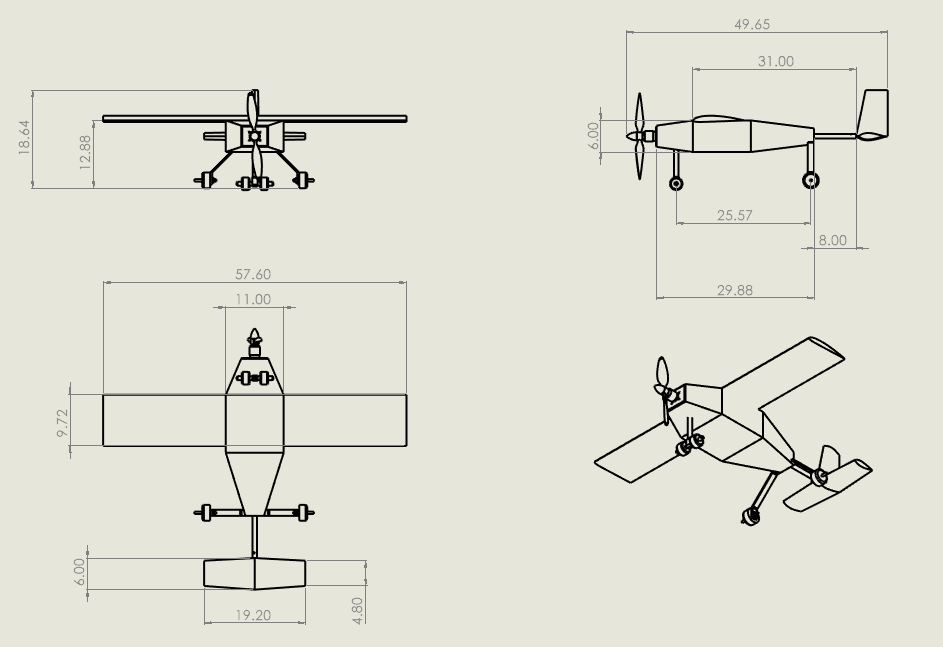
\includegraphics[width=\textwidth]{Images/goon-2D-2.png}
        \caption{Aircraft 2D-Sketch}
        \label{fig:Aircraft_2D}
    \end{subfigure}
    \hspace{\fill}
    \begin{subfigure}[b]{0.49\textwidth}
        \centering
        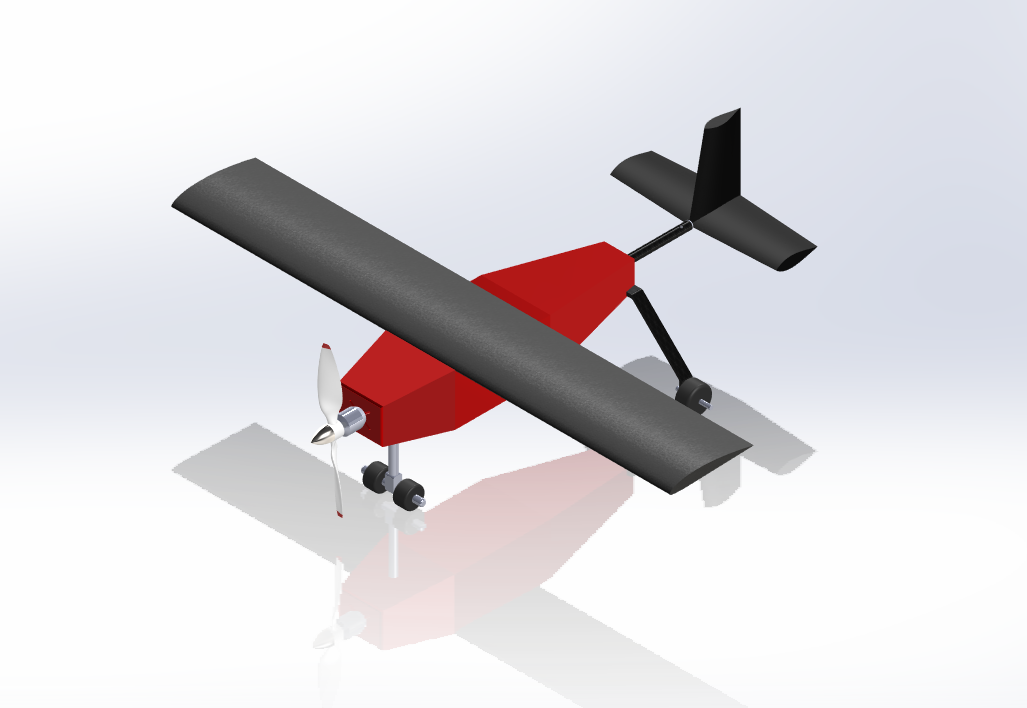
\includegraphics[width=\textwidth]{Images/goon-3D.PNG}
        \caption{Aircraft 3D-CAD}
        \label{fig:Aircraft_3D}
    \end{subfigure}
    \hspace{\fill}
    \caption{Preliminary Design}
    \label{fig:score}
    \vspace{1em}
\end{figure}

\begin{atb}{Preliminary Aircraft Dimensions}{tab:Dims}{r l @{\hskip 25pt} r l}
    \cellcolor{iitred} %\
    Empty Weight & \cellcolor{white}6.65 lb & \textcolor{white}{Payload Weight} & \cellcolor{white}2.85 lb  \\
    %
     %\
    \cellcolor{iitred}Structural Weight & \cellcolor{white}3.68 lb & \cellcolor{iitred} \textcolor{white}{Total Weight} & \cellcolor{white}9.50 lb  \\
    %
    \cellcolor{iitred}Wing Area & 560 in$^2$ & \cellcolor{iitred} \textcolor{white}{Wingspan} & 57.6 in \\
    %
    \cellcolor{iitred}{Horizontal Tail Area} & 
    115 in$^2$ & \cellcolor{iitred} \textcolor{white}{Horizontal Tail Span} & 19.2 in \\
    %
     %
    \cellcolor{iitred}{Vertical Tail Area} & 
    44.7 in$^2$ & \cellcolor{iitred} \textcolor{white}{Vertical Tail Height} & 8.76 in \\
    %
    \cellcolor{iitred}Fuselage Length & 30 in & \cellcolor{iitred} \textcolor{white}{Fuselage Width} & 11 in
\end{atb}

\subsection{Propulsion Selection}
    Propulsion requirements were determined from the desired thrust-to-weight ratio and endurance. The required thrust for takeoff and cruise speeds were determined based on the aerodynamic parameters and structural limitations of the preliminary aircraft design. 
    eCalc, a propulsion 
    \begin{wraptable}{r}{}
    % \centering
    \begin{tabular}{cccccr}
    \rowcolor{iitred}\color{white}Criteria & \color{white}Points & \color{white}Power 60A & \color{white}SII-4020 & \color{white}X5-400\\
    \color{white}\cellcolor{iitgray}T/W  & 45 & 3 & 1 & 2\\
    \color{white}\cellcolor{iitgray}Flight Time & \cellcolor{gray!25}30 & \cellcolor{gray!25}2 & \cellcolor{gray!25}3 & \cellcolor{gray!25}1\\
    \color{white}\cellcolor{iitgray}Weight & 35 & 2 & 1 & 3 \\\hlineB{2.5}
    \color{white}\cellcolor{iitgray}Total & \cellcolor{gray!25}100 & \cellcolor{gray!25}265 & \cellcolor{gray!25}170 & \cellcolor{gray!25}225\\     
    \end{tabular}
    \caption{ Propulsion Selection Matrix}
    \label{tab:hss}
\end{wraptable} 
system analysis software, was used to find battery, propeller, and motor configurations that met the targeted thrust, cruise speed, and endurance requirements. A selection matrix was used to determine the motor for the aircraft, shown in Table \ref{tab:hss}. All configurations are predicted to have a thrust-to-weight ratio above 1.00 and mixed flight time of at least ten minutes.
% can't specify "in pounds" there. W/S is dimless. Sadge.

\subsection{Wing and Jamming Antenna Integration}
%\begin{wrapfigure}{r}{.3\linewidth}
    % \vspace{-1em}
   % \centering
    %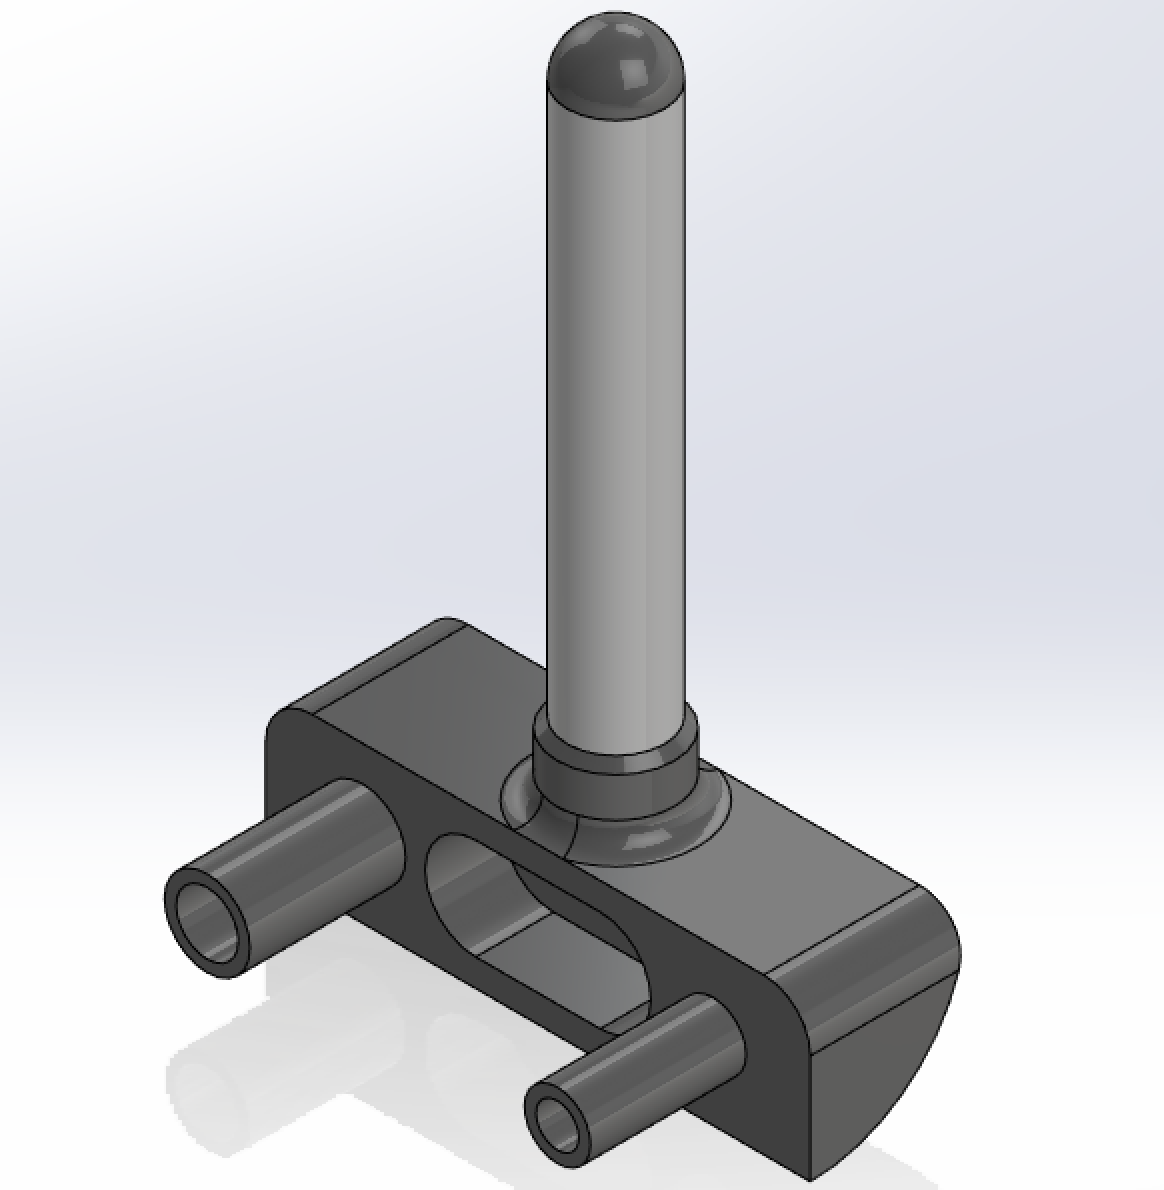
\includegraphics[width=\linewidth]{Images/ant_CAD.png}
   % \caption{Antenna Connector}
   % \label{fig:Connector}
   % \vspace{0.3em}
%\end{wrapfigure}
With the requirement of detachable wing sections designed for rapid assembly and high structural strength, a fast attachment method was necessary for mounting the wings. Side mounting of the wings was chosen to maximize available wingspan and allow for ease of wing section \begin{wrapfigure}{r}{.3\linewidth}
    % \vspace{-1em}
   \centering
    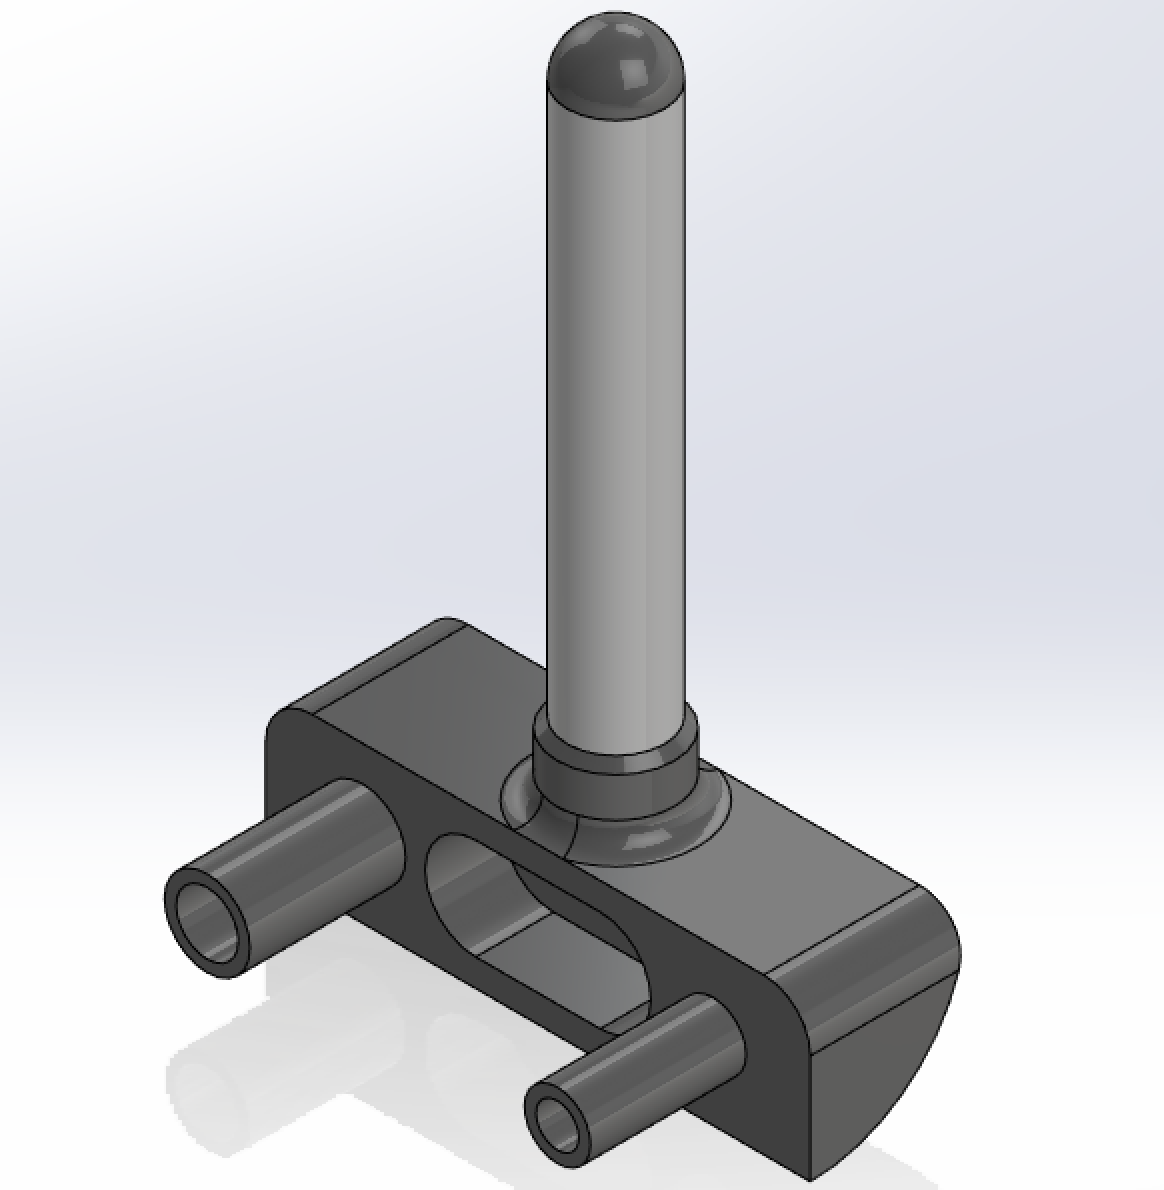
\includegraphics[width=\linewidth]{Images/ant_CAD.png}
   \caption{Antenna}
   \label{fig:ant}
   % \vspace{0.3em}
\end{wrapfigure}
manufacturing. Each wing will be mounted by sliding the two wing spars into two hollow shafts in the fuselage. Locking pins will secure the wing to the fuselage while allowing for strong structural coupling. Similarly, the antenna (see Figure \ref{fig:ant}) will be mounted using a 3D-printed component that will slot into the hollow carbon fiber spars at the wingtips. An adapter must be made for each side, as the spars are not of the same inner diameter. A counterweight will be used on the opposite wingtip to improve lateral stability. Additional testing must be done to test acceptable lengths based on final design, wind interference, and manufacturing.

% \begin{figure}[htb!]
%     % \vspace{-1.5em}
%     \hspace{\fill}
%     \begin{subfigure}[b]{0.49\textwidth}
%         \centering
%         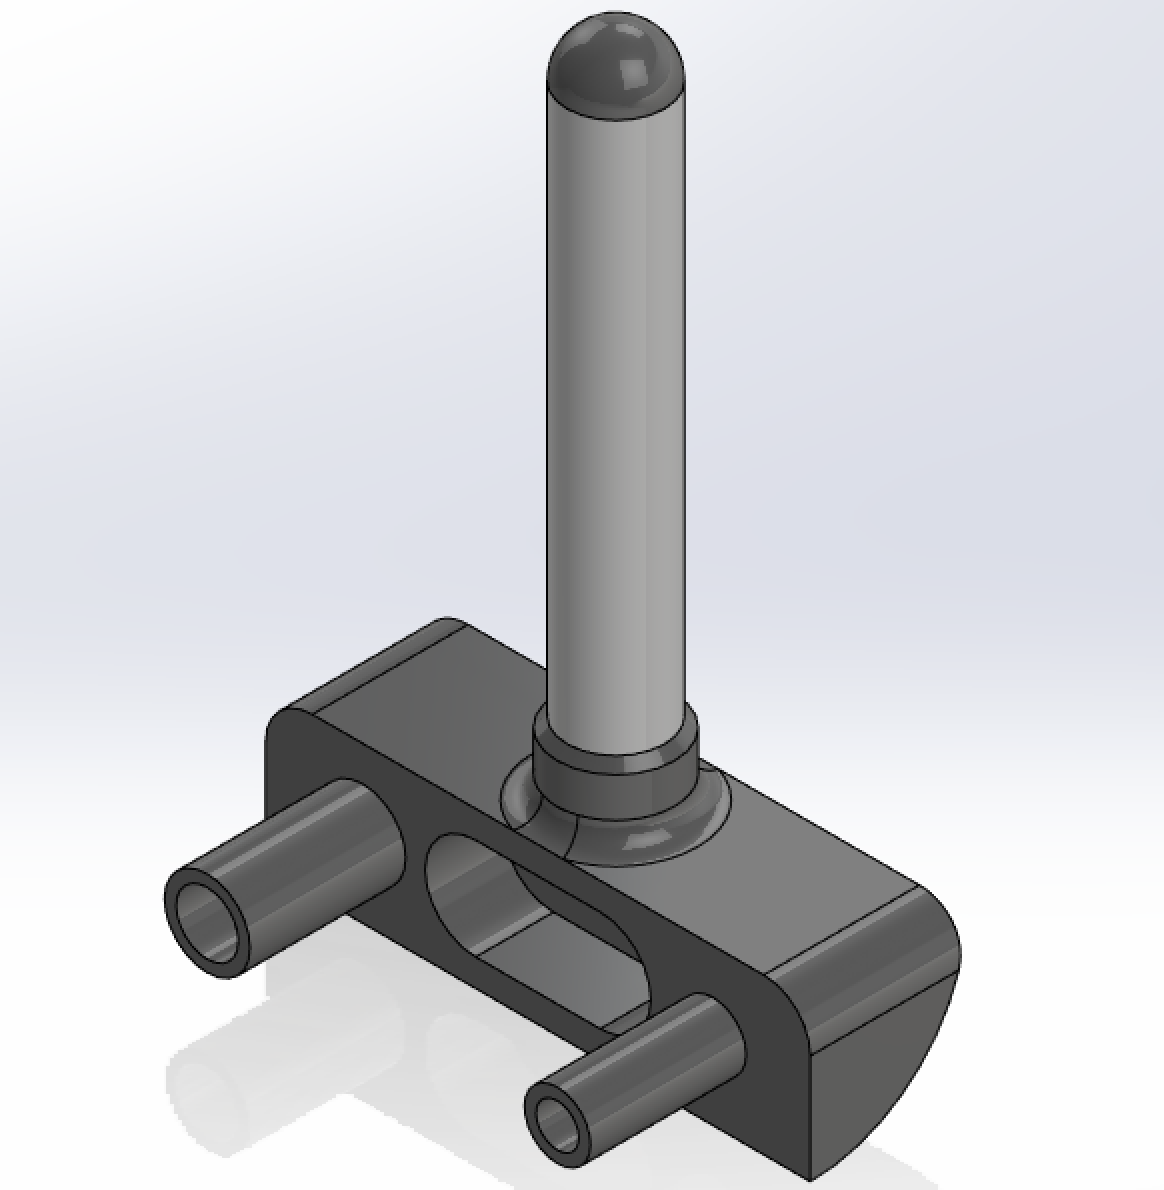
\includegraphics[width=\textwidth]{Images/ant_CAD.png}
%         \caption{Conceptual Connector}
%         \label{fig:Connector}
%     \end{subfigure}
%     \hspace{\fill}
%     \begin{subfigure}[b]{0.42\textwidth}
%         \centering
%         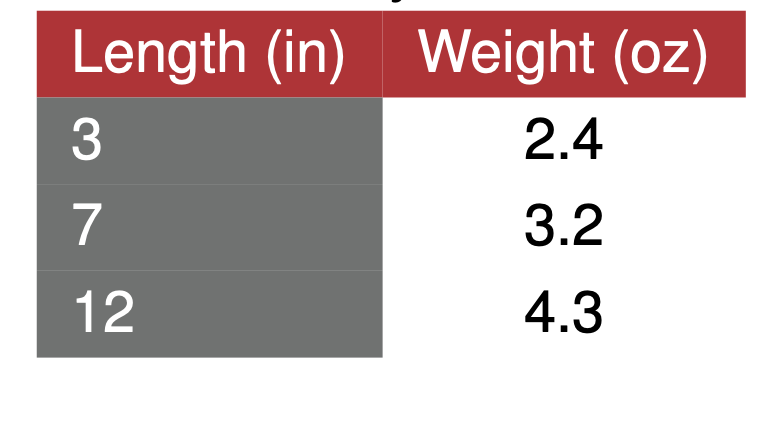
\includegraphics[width=\textwidth]{Images/ant_sel.png}
%         \caption{Aircraft 3D-CAD}
%         \label{fig:score_3d}
%     \end{subfigure}
%     \hspace{\fill}
%     \caption{Preliminary Design}
%     \label{fig:score}
%     \vspace{1em}
% \end{figure}



    % \begin{figure}
    %     \centering
    %     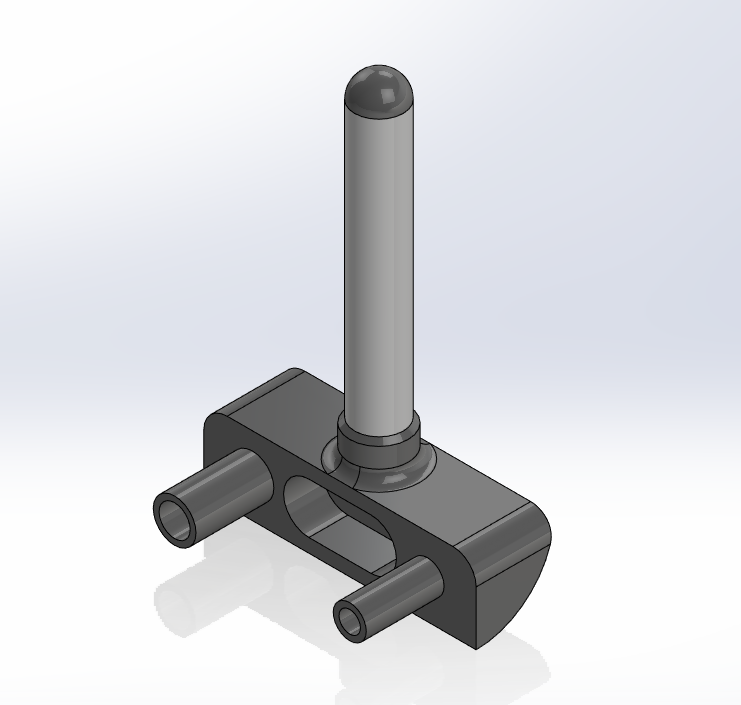
\includegraphics[]{Images/AntennaWConnector.png}
    %     \caption{Antenna Connector with 7 inch connector}
    % \label{fig:Connector}
    % \end{figure}